\section{Building and Testing CrashSimulator}
\label{SEC:architecture}

\begin{figure}[t]
  \center{}
  \fbox{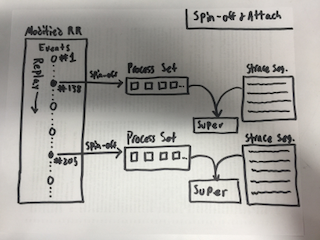
\includegraphics[scale=.75]{architecture}}
  \caption{Diagram illustrating CrashSimulator's Architecture.  During the
    course of a single rr execution, clone process sets are generated at
    specific rr events.  A CrashSimlator supervisor process attaches to
    these process sets and uses a strace-style system call listing to feed
    subsequent system call activity and inject unusual environmental
    conditions.}
  \label{figure:architecture}
\end{figure}

CrashSimulator's testing process for any application
consists of launching it as a child process and
interceeding in its execution at appropriate times in order to simulate the
results and side effects of any system call the application might make.
Its testing approach requires two pieces of
functionality, starting with a way to maintain
repeatable execution of the application.  This ensures that
the system call sequence required by the anomaly being tested is reached.
The second element required for its test protocol is a
way to interpose on an execution in order to modify the results and side
effects of system calls to reflect the environmental
anomaly.  Our current iteration of
CrashSimulator uses a modified version of {\tt rr} to handle the first
requirement and a custom process supervisor to handle the
second.

The {\tt rr} debugger is an excellent candidate
for handling repeatable executions
because of it can
record and replay applications quickly and accurately out right out of the
box.  This makes the tool valuable for both human-in-the-loop and automated
continuous integration/continuous deployment testing scenarios.  Replay
executions occur as a sequence of ``events'' that map to application
events like system calls and signals.  We modified {\tt rr} so that it
could be made to run to a specific event corresponding to a specific system
call and then generate clones of the set of processes being replayed at that
point in time.  These cloned process sets exist entirely separately from
{\tt rr}, allowing the tool to continue through
its replay process to the next
designated event.  One {\tt rr} replay execution can spin
off as many process sets as may be required to perform the set of tests
configured by the user.

Process sets generated by {\tt rr} are created in a stopped state and
remain until they are attached to and utilized by a CrashSimulator
supervisor.  Each process set has its own supervisor process to inject
its configured environmental anomaly.  The
supervisor wakes up the process set it is managing and simulates any
subsequent system calls it makes.  The data necessary for this
simulation is
supplied as a system call listing formatted after the style of {\tt strace}
output, that describes the results and side effects for each system
call. The output is engineered in such a way to contain the
elements required to reflect the
desired environmental anomaly.  Supervisors can complete this
process independently of one another, which lends a
high degree of speed and
parallelism to the whole CrashSimulator testing process.
